\documentclass[a4paper, 11pt, oneside]{scrartcl}
\usepackage[utf8]{inputenc}      		% Required for simple use of ö,ä,ü
\usepackage{graphicx}					% Required for use of figures
\usepackage{textcomp}					% Required to write ° with \textdegree
\usepackage{amsmath}					% Required for advanced formulas
\usepackage{siunitx}					% Required for scientific notation of numbers (and more)
\usepackage{subcaption}					% Required for sufigures
\usepackage{lettrine}					% Required for large letters at beginning of chapter
\usepackage{sectsty}					% Required for centered section captions 
\usepackage{fancyhdr}					% Required for modified title page
\usepackage[export]{adjustbox}
\usepackage{xcolor}
\definecolor{TUMblue}{RGB}{0,101,189} 
\usepackage{geometry}
\usepackage{amsfonts}
\usepackage{amssymb}
\usepackage{hyperref}
\usepackage{fontawesome5}
\hypersetup{colorlinks=true,linkcolor=blue,urlcolor=blue}
\geometry{left=12.5mm, top=20mm, bottom=25mm, right=12.5mm}

\pagestyle{fancy} 
\fancyhf{}
\renewcommand{\headrulewidth}{0pt}
\renewcommand{\footrulewidth}{0.4pt}
\fancyfoot[R]{\thepage}
\fancyfoot[L]{\fontsize{8}{8} \selectfont \textit{Multilevel Monte Carlo Methods for Uncertainty Quantification (TUM, SS 2026)}}
 
\fancypagestyle{empty}{
\fancyhf{}
\fancyhead[R]{ 
\includegraphics[valign=c,width=0.13\textwidth]{TUM_Logo_blau_rgb_p.png}  }
\fancyhead[L]{ 
{\color{TUMblue}
    \begin{tabular}{@{}l @{}}
    Department of Mathematics \\
    TUM School of Computation, Information and Technology \\
    Technical University of Munich 
\end{tabular}   
}
 }
\renewcommand{\headrulewidth}{0pt}
\renewcommand{\footrulewidth}{0.4pt}
\fancyfoot[R]{\thepage}
\fancyfoot[L]{\fontsize{8}{8} \selectfont \textit{Multilevel Monte Carlo Methods for Uncertainty Quantification (TUM, SS 2026)}}
}
%%%%%%%%%%%%%%%%%%%%%%%%%%%%%%%%%%%%%%%%%%%%%%%%%%%%%%%%%

% Title Page 
\title{ Efficient White Noise Sampling and Coupling for Multilevel Monte Carlo with Nonnested Meshes}
\author{M. Croci, M.B. Giles, M.E. Rognes and P.E. Ferrel}
\date{Seminar Report by Federico Riva\\
\textit{Multilevel Monte Carlo Methods for Uncertainty Quantification} }

\newtheorem{lemma}{Lemma}
\newtheorem{proof}{Proof}
\newtheorem{definition}{Definition}

% Start of document 
\begin{document}
\maketitle
\thispagestyle{empty}

\section{Summary}
In many applications it is required to generate samples from specific points of a Gaussian random field. This produces a Gaussian random vector with specific distribution parameters, namely the mean vector and the covariance matrix.
Algorithms like the Box-Muller let us easily sample from a standard normal distribution. While the desired mean can be achieved via the summation of the mean vector, the right covariance is quite more involved. In the general case, given the covariance matrix of a Gaussian vector it is necessary an expensive Cholesky factorization. 
However, in the particular case presented by this article the covariance matrix is the mass matrix of a finite element method. The main idea to make the sampling more efficient is to exploit the assembling of the global mass matrix as a linear combination of all mass matrices associated to each element of the mesh. Due to linearity it is possible to factorize the smaller mass matrices of the elements instead of the more extended global one. 

\section{Methods - The Article}
Given the following elliptic PDE with random coefficient \(u\)
\begin{equation}
\begin{cases}
-\nabla \cdot ( e^{u(x,w)} \nabla q(x,w) ) = 1, \quad x \in G=[-0.5,0.5]^d, \quad \ w \in \Omega \\ \quad q(x,w) = 0, \hspace{3cm} x \in \partial G, \quad \ w \in \Omega
\end{cases}
\end{equation}
we are interested in estimating the expected value of the \(L^2\)-norm of the solution \(q\)
\begin{equation}
\mathbb{E}\left[ \|q\|_{L^2(G)} \right] = \int_\Omega \|q\|_{L^2(G)}(w) d \mathbb{P}(w),
\end{equation}
This task can be seen as computing the expected value of a real valued random variable \( \mathcal{P}:= \|q\|_{L^2(G)} : \Omega \rightarrow \mathbb{R}.\) Let's assume \(u\) is a Gaussian random field with zero mean and Matérn covariance \(\mathcal{C}\)
\begin{equation}
\mathcal{C}(x,y) = \frac{\sigma^2}{2^{\nu -1} \Gamma(\nu)}(\kappa r)^\nu K_{\nu}(\kappa r), \quad r =\|x-y\|_2, \quad \kappa = \frac{ \sqrt{8 \nu} }{\lambda}, \quad x,y \in D
\end{equation} 
where \( \sigma^2, \nu, \lambda > 0\) are respectively the variance, smoothness and correlation length of the random field. \( K_{\nu}\) is the modified Bessel function of second kind [2]. \\
In practice, samples of \(u\) are needed only at discrete locations \( \texttt{x}_1, \dots , \texttt{x}_m \in D\) and a simple sampling strategy consist of drawing realizations of a Gaussian vector \( \texttt{u} \sim N(0,C) \) with \( \texttt{u}_i = u(\texttt{x}_i) \) and covariance matrix \( C_{ij}  = \mathbb{E}[u(\texttt{x}_i)u(\texttt{x}_j)] \in \mathbb{R}^{ m \times m} \).
The easiest approach is the most computationally expensive as it requires the factorization of a dense covariance matrix which has a computational complexity of \( \mathcal{O}(m^3) \). We can use Algorithms like Box-Muller [3] to sample form a standard Gaussian vector \( \mathtt{z} \sim N(0,I) \), \( I \in \mathbb{R}^{n \times n}\), and the factorization of \( C = HH^T\), with \( H \in \mathbb{R}^{ m \times n} \), gives the desired sample \( \texttt{u} \) as \( \texttt{u} = H \texttt{z} \)  since
\begin{equation}
\mathbb{E} [ \texttt{u} \texttt{u}^T ] = \mathbb{E} [ H \texttt{z} (H \texttt{z})^T ] = H I H^T = C. 
\end{equation}
Among all the other methods that exist for the generation of random filed samples (Karhunen-Loéve expansion, circulant embedding etc... ) we choose a particular one which exploits both the use that we will do of the generated sample, as part of a finite element method, and its specific covariance function. \\
In fact, a standard result in the SPDE theory shows that a Gaussian random field with Matérn covariance satisfies the following elliptic PDE
\begin{equation}
(I - \kappa ^{-2}\Delta)^k u(x,w) = \dot{W}(x,w) \quad x \in \mathbb{R}^d, \ w \in \Omega, \quad \nu = 2k -d/2>0,
\end{equation}
where \(\dot{W}\) is Gaussian white noise defined on \(\mathbb{R}^d\). For simplicity we will consider the case \(k=1\). 
Nevertheless it is not feasible to solve the PDE on the whole \(\mathbb{R}^d\), hence we restrict ourself on a domain \(D\) such that \( G \subset D\). Some boundary conditions are needed, for example homogeneous Dirichlet, but if D is sufficiently large, in the sense that the distance between \( \partial G\) and \( \partial D\) is larger that the correlation length \(\lambda\), the error induced by truncating \( \mathbb{R}^d\) to \(D\) is negligible.
\begin{definition}[White Noise]
Let \( D \subset \mathbb{R}^d \) be an open domain, \(\dot{W} \in \mathcal{L}( L^2(D), L^2(\Omega,\mathbb{R})) \) 
 i.e a linear functional on \(L^2(D)\) such that it induces a square integrable real valued random variable and for any collection of function \( \{ \phi_i \} \subset L^2(D) \), if we let \( b_i = \langle \dot{W}, \phi_i \rangle\), \( \{ b_i\}\) are joint Gaussian random variables with zero mean and covariance 
\begin{equation}
\mathbb{E}[b_i b_j] = \mathbb{E}\left[ \int_D \phi_i(x)\dot{W}(x) dx \int_D \phi_j(y)\dot{W}(y) dy \right]= \int_{D \times D} \phi_i(x)\phi_j(y)\underbrace{\mathbb{E} \left[ \dot{W}(x) \dot{W}(y)\right]}_{\delta(x-y)} dxdy = ( \phi_i,\phi_j). 
\end{equation}
\end{definition}
This sampling technique gives us a random field sample with the right covariance function and choosing the same FEM space, restricted to our smaller domain \(G\) to solve the original PDE, we have for free the value of the random field at the right nodes. \\
However, this strategy \textit{moves} the sampling problem on the realization of the White Noise as right hand side. 
To generate the random filed sample, i.e. solve the SPDE, we choose a suitable finite element approximation subspace \( V_h^D = \text{span} \{\phi_1, \dots, \phi_m \} \subset H^1_0(D)\) like the linear Lagrange basis functions. As mentioned, we choose a mesh and a function space that will allow us to solve not only the SPDE but also the elliptic PDE with random coefficient.\\
Since \(G \subset D\), we can take two nested meshes, \( G_h \subset D_h\), and choosing the same function space obtain 
\begin{equation}
 V_h^G := \{ \phi_i \in V_h^D | \ \text{supp}(\phi_i) \subset G \} \subset V_h^D, \quad |V_h^G| = m' \quad \text{and}\quad V_h^G \subset H^1_0(G) \cap H^1_0(D).
\end{equation}
The discretized weak form reads as follows:
\begin{equation}
(u_h,v_h) + \kappa^{-2}( \nabla u_h,\nabla v_h) = \langle \dot{W}, v_h \rangle \quad \forall \ v_h \in V_h^D
\end{equation}
The coefficients of the basis function expression for \(u_h\), i.e. the \( \texttt{u}_i\) such that \( u_h = \Sigma_{i=1}^m \texttt{u}_i \phi_i \), are given by the solution of the following linear system
\begin{equation}
A \texttt{u} = b, \quad \text{with} \ A_{ij} = (\phi_i,\phi_j) + \kappa^{-2} (\nabla \phi_i,\nabla \phi_j), \quad \text{b}_i = \langle \dot{W}, \phi_i \rangle \quad i \in 1, \dots, m. 
\end{equation}
The discretized version of the right hand side is a Gaussian vector by definition of white noise 
\begin{equation}
b \in N(0,M),\ M_{ij} = (\phi_i,\phi_j).  
\end{equation}
Sampling white noise realization can thus be accomplished by sampling a Gaussian vector of mass matrix covariance. 
This result, as presented so far, does not constitute any improvement over the straightforward sampling of the Gaussian vector with covariance matrix obtained from the discretization of the Matérn random field since an expensive Cholesky factorization of \(M\) is still necessary. 
The crucial difference is how the matrix \(M\) can be assembled as linear combination of the element-wise mass matrices. \\
In case of a mesh composed by \(n\) elements and \(m_e\) degrees of freedom on each element the local mass matrices \(M_e\) are of size \( m_e \times m_e \) and  computed on each mesh element  \(e\). The overall aggregation to form the global mass matrix \(M\) can be written 
\begin{equation}
M = L^T \text{diag}(M_e)L,
\end{equation}
where: \(\text{diag}(M_e)\) is a block diagonal matrix of size \( nm_e \times nm_e\), \(L\) is a Boolean assembling matrix of size \( nm_e \times m \) such that \( L^T = [L_1^T, \dots , L_n^T]\) and \( \{ L_e \}_{e=1}^N \) are Boolean matrices of size \( m_e \times m\) that encode the local-to-global map. 
We can now factorize each local mass matrix \( M_e\) with Cholesky factorization to obtain \( M_e = H_e H_e^T\) for each element \(e\).
We then have 
\begin{equation}
M = L^T \text{diag}(H_e H_e^T)L = (L^T \text{diag}(H_e) )( L^T \text{diag}(H_e))^T = HH^T.
\end{equation}
With \( H:=L^T \text{diag}(H_e)\) we can sample \( \texttt{b} \) by computing
\begin{equation}
\texttt{b} = Hz, \quad \text{z} \sim N(0,I), \quad \text{z} \in \mathbb{R}^{m_en}
\end{equation}
since
\begin{equation}
\mathbb{E}[\text{b}\text{b}^T] = H \mathbb{E}[ \text{z}\text{z}^T]H^T =\underbrace{(L^T \text{diag}(H_e) )I( L^T \text{diag}(H_e))^T}_{(m \times nm_e) ( nm_e \times nm_e) (nm_e \times m)= (m \times m)} = M.
\end{equation}
This strategy allows the splitting of a large global sampling problem into separate small local sampling problems. In fact, if for each element \(e\) we write \( \text{z}_e \sim N(0,I) \) be a small standard Gaussian vector of length \(m_e\), we can write 
\begin{equation}
\text{b} = H \text{z} = \sum_{e=1}^n L_e^TH_e \text{z}_e = \sum_{e=1}^n L_e^T \text{b}_e , \quad \text{b}_e \sim N(0,M_e) .
\end{equation}
The problem of sampling a global mass matrix covariance Gaussian vector eventually reduces to the sampling of \(n\) independent local mass matrix covariance Gaussian vectors. This is immediately parallizable and from the computational point of view the overall cost is \( \mathcal{O}(m_e^3n)\). 
In the special case of an affine linear transformation to the reference element, such as for the linear Lagrange test functions, this operation can be made even more efficient by noting that the local mass matrices on each element are always the same up to a multiplicative factor \[ M_e / |e|=\text{const} \ \text{for all} \ e,\] where \( |e|\) is the size of the element. It is therefore sufficient to factorize a single local mass matrix and store its Cholesky factor which further reduces the computational cost to \( \mathcal{O}(m_e^3). \) \\
Even though we have developed an efficient technique to realize sample of the right hand side of the SPDE we still have to solve it to be able to generate a single sample of the Matérn random filed. Moreover after this step has been done have to solve the elliptic PDE with random coefficient to estimate the quantity of interest, i.e. the \(L^2\)-norm of the solution \(q\).\\
As previously discussed, a suitable choice of nested meshes and function spaces on \(G\) and \(D\) yields
\begin{equation}
\int_G e^{u_h(x,w)} \nabla v_h(x) \nabla q_h(x,w) dx = \int_G 1 \ v_h(x) dx \quad \forall \ v_h \in V_h^G \subset V_h^D
\end{equation}
The coefficients of the basis function expression for \(q_h\), i.e. the \(\texttt{q}_i\) such that \(q_h = \Sigma_{i=1}^{m'} \texttt{q}_i\phi_i \) are given by the solution of the following linear system
\begin{equation}
A \texttt{q} = b, \quad \text{with} \ A_{ij} = (e^{u_h(\cdot,w)} \nabla \phi_i,\nabla \phi_j), \quad b_i = (1,\phi_i) \quad \phi_1, \dots, \phi_{m'}.
\end{equation}
Even if we use the most efficient pre-conditioner to solve both PDEs the computational cost to solve both of them is \( \mathcal{O}(m)\), since \( m \approx m'\).
In many application of interest such cost for each sample makes a standard Monte Carlo method too expensive to be used in practice since the statistical unbiased estimator
\begin{equation}
E^{MC}[\mathcal{P}] \approx E^{MC}[\mathcal{P}_h] = \frac1N \sum_{i=1}^N \|q_h(\cdot,w_i) \|_{L^2(G)} = \frac1N \sum_{i=1}^N \sqrt{\texttt{q}(w_i)^T M \texttt{q}(w_i)}
\end{equation}
has a slow variance convergence rate.
The standard solution in this circumstances is to choose a Multilevel Monte Carlo method instead. 
Consider a sequence of meshes with decreasing elements diameters \( \{h_l\}_{l=1}^L\) labelled by \( l = 1, \dots L\); MLMC method is implemented as
\begin{equation}
E^{MLMC}[\mathcal{P}] \approx  E^{MLMC}[\mathcal{P}_{h_L}] = \sum_{l=1}^L \left[ \frac{1}{N_l}  \sum_{n=1}^{N_l}  \| q_{h_l}(w_l^n) \|_{L^2(G)}-\|q_{h_{l-1}}(w_l^n) \|_{L^2(G)} \right]
\end{equation}
where \( w_l^n \in \Omega\) is the \(n\)-th sample point on level \(l\). \\
When using \(h\)-refinement, we construct the MLMC mesh hierarchies \( \{ D_{h_l}\}_{l=1}^L\), and therefore \( \{ G_{h_l}\}_{l=1}^L\), in such a way that \(  G_{h_l} \) is embedded within \( D_{h_l}\) for all \(l\), but \(  G_{h_{l-1}} \) and \(  D_{h_{l-1}} \) are not necessarily nested in their respective higher levels, i.e. \( D_{h_{l-1}} \not\subset D_{h_l} \).
The improved efficiency of the Multilevel Monte Carlo estimator compared to the standard Monte Carlo method relies on a suitable balance between computational cost and variance across the discretization levels.
On the coarse levels (\(l\) small), the variance of the correction terms is relatively large, and therefore a large number of samples is required to estimate their expectation accurately. However, each sample is inexpensive since it is computed on a coarse mesh.
On the fine levels (\(l\) large), the computational cost per sample increases due to the finer discretization. Nevertheless, only a relatively small number of samples is needed because the variance of the correction
\[
Y_l(w) :=
\|q_{h_l}(w)\|_{L^2(G)}
-
\|q_{h_{l-1}}(w)\|_{L^2(G)}
\]
decreases. This variance reduction is achieved by coupling the two approximations through the same realization \(w_l^n\), namely by evaluating both
\(
\|q_{h_l}(w_l^n)\|_{L^2(G)}
\ \text{and} \
\|q_{h_{l-1}}(w_l^n)\|_{L^2(G)}
\)
at the same sample point. \\
The variance of the correction term satisfies
\[
\operatorname{Var}(Y_l)
=
\operatorname{Var}(Q_l-Q_{l-1})
=
\operatorname{Var}(Q_l)
+
\operatorname{Var}(Q_{l-1})
-
2\,\operatorname{Cov}(Q_l,Q_{l-1}), \ \text{where} \ Q_l := \|q_{h_l}(w)\|_{L^2(G)}.
\]
From an intuitive viewpoint we can say that since \(Q_l\) and \(Q_{l-1}\) are computed from the same realization of the random input, and \(u_{h_l}(\cdot,w) \approx u_{h_{l-1}}(\cdot,w)\), then, due to the stability of the Finite Element Method, \(q_{h_l}(\cdot,w) \approx q_{h_{l-1}}(\cdot,w)\). Hence,the values of \(Q_l\) and \(Q_{l-1}\) are strongly correlated. 
Consequently,
\[
\operatorname{Cov}(Q_l,Q_{l-1})
\approx
\sqrt{\operatorname{Var}(Q_l)\operatorname{Var}(Q_{l-1})},
\]
which implies a substantial cancellation in the expression above and yields a much faster convergence rate with respect to the standard Monte Carlo due to
\(
\operatorname{Var}(Y_l)
\ll
\operatorname{Var}(Q_l).
\)  \\
We now consider the case in which coupled Matérn field realization are needed in a MLMC setting. As we have discussed the key part to achieve an actual variance reduction is the sampling of \( u_l(x,w) \) and \( u_{l-1}(x,w)\) for the same \( w \in \Omega.\)\\
Since the only stochastic part in the generation of the random filed is white noise forcing term is it sufficient to use the same white noise sample on both levels to enforce the coupling requirement. \\
More precisely, let \(V_{h_l}^D\) and \( V_{h_{l-1}}^D\)  be the finite element spaces on levels \(l \) and \(l-1\) for \(l>1\).
We consider the following to discritezed variational problems coupled by a common white noise sample. Consider \( V_{h_l}^D = \text{span}(\phi_1^l, \dots, \phi_{m_l}^l)\) and  \( V_{h_{l-1}}^D = \text{span}(\phi_1^{l-1}, \dots, \phi_{m_{l-1}}^{l-1} )\) such that for \( w_l^n \in \Omega\)
\begin{equation}
\begin{aligned}
(u_{h_l},v_{h_l}) + \kappa^{-2}( \nabla u_{h_l},\nabla v_{h_l}) &= \langle \dot{W}, v_{h_l} \rangle(w_l^n) \quad \forall \ v_{h_l} \in V_{h_l}^D \\
(u_{h_{l-1}},v_{h_{l-1}}) + \kappa^{-2}( \nabla u_{h_{l-1}},\nabla v_{h_{l-1}}) &= \langle \dot{W}, v_{h_{l-1}} \rangle(w_l^n) \quad \forall \ v_{h_{l-1}} \in V_{h_{l-1}}^D
\end{aligned}
\end{equation}
where the terms on the right hand side are coupled in the sense they are centred Gaussian random variables with covariance function \( \mathbb{E}[ \langle\dot{w},v_l\rangle \langle \dot{w}, v_{l-1}\rangle ]=(v_l,v_{l-1}).\)\\
Let \( \texttt{u}_l \in \mathbb{R}^{m_l}\) and \( \texttt{u}_{l-1} \in \mathbb{R}^{m_{l-1}}\) be the vectors of coefficients of \(u_l\) and \(u_{l-1}\) respectively. As previously discussed the unknowns are given by a suitable linear system
\begin{equation}
A \texttt{u} = b \in \mathbb{R}^{m_l + m_{l-1}} \quad \text{with} \ 
\begin{pmatrix}
A^l & 0 \\
0 & A^{l-1} 
\end{pmatrix} 
\begin{pmatrix}
\texttt{u}_l \\
\texttt{u}_{l-1}
\end{pmatrix} =
\begin{pmatrix}
b_l \\
b_{l-1}
\end{pmatrix}.
\end{equation}
The vector \( b\) is the white noise sample and \( b_i = \langle \dot{W}, \phi_i^l \rangle \) for \( i = 1, \dots, m_l \), while \( b_{m_l+j} =  \langle \dot{W}, \phi_j^{l-1} \rangle \) for \( j = 1, \dots, m_{l-1}. \)
By white noise definition \( \mathbb{E}[ b_i b_j] = \mathbb{E}[\langle \dot{W}, \phi_i^l \rangle \langle \dot{W}, \phi_j^{l-1} \rangle]  \), hence b is a Gaussian random vector in \( \mathbb{R}^{m_l + m_{l-1}}\)
\begin{equation}
b \sim N(0,M), \quad \text{with} \ M = \begin{pmatrix}
M^l & M^{l,l-1} \\
(M^{l,l-1})^T & M^{l-1}
\end{pmatrix},
\ M_{ij}^{l,l-1} = ( \phi_i^{l}, \phi_j^{l-1} ) \ \text{and} \ M_{ij}=(\phi_i^l,\phi_j^l)
\end{equation}
where \( M^{l,l-1} \in \mathbb{R}^{m_l \times m_{l-1}} \), \(M^{l-1} \in \mathbb{R}^{m_{l-1} \times m_{l-1}} \) and \( M^l \in \mathbb{R}^{m_l \times m_l} \).
If we were using independent samples then the off diagonal blocks of \(M\) would vanish. 
In this case there is not an immediate linear combination which assembles M. Hence, we cannot directly replicate the previous efficient sampling technique.
Moreover, to assemble \( M^{l,l-1}\) we need to compute integral involving basis function which are defined over different, possibly non-nested, meshes. This task is non-trivial due to the lack of smoothness of piecewise polynomial functions.
The solution for such problems is use a so called super-mesh.
\begin{definition}[Super-mesh] Let \(D\) be a compact subset of \(\mathbb{R}^d\), and let \( T_a\),\(T_b\) be two tessellations of \(D\). A super-mesh \( S\) of \( T_a\) and \(T_b\) is a common refinement of both meshes.
More specifically, \( S\) is a triangulation of \(D\) such that
\begin{itemize}
\item[1] \(\text{vertices}(T_a) \cup \text{vertices}(T_b) \subseteq \text{vertices}(S)\)
\item[2] \(\text{volume}(e_S \cap e) \in \{ 0,\text{volume}(e_S) \} \ \forall e_s \in S, \ e \in (T_a \cup T_b) \)
\end{itemize}
\end{definition}
Our strategy relies on constructing a super-mesh over \(D_{h_l}\) and \( D_{h_{l-1}}\). Note that each super-mesh element is formed by the intersection of exactly one pair of parent elements, \(e_l \in D_{h_l}\) and \( e_{l-1} \in D_{h_{l-1}}\). Consequently, we only need to consider the basis functions that are non-zero over both \(e_l\) and \( e_{l-1}\). Let \(m_{e_l} \) and \(m_{e_{l-1}}\) denote the number of degrees of freedom associated with the finite element spaces \(V_{h_l}^D\) and \( V_{h_{l-1}}^D \) restricted to the elements \( e_l\) and \( e_{l-1} \), respectively. Under these conditions, only the inner products between these \(m_e = m_{e_l} + m_{e_{l-1}}\) basis functions will be non-zero. \\
The mass matrix over an element of the super-mesh is constructed as
\begin{equation}
M_e = \begin{pmatrix}
M_e^l & M_e^{l,l-1} \\
(M_e^{l,l-1})^T & M_e^{l-1} 
\end{pmatrix} \in \mathbb{R}^{ m_e \times m_e }, \quad ( M_e^{l,l-1})_{ij} = \int_e \phi_i^l \phi_j^{l-1} dx,
\end{equation}
where \( \{ \phi_i^l \}_{i=1}^{m_{e_l}} \) and \( \{ \phi_j^{l-1} \}_{j=1}^{m_{e_{l-1}}} \) are the sets of the basis functions that have non zero support over \(e\). 
We can now use the Boolean assembling matrices \(L^l\) and \( L^{l-1} \) corresponding to the elements of the two original meshes
\begin{equation}
M = \begin{pmatrix}
(L^l)^T & (L^{l-1})^T
\end{pmatrix} 
\begin{pmatrix}
\text{diag}(M_e^l) & \text{diag}(M_e^{l,l-1})\\
\text{diag}(M_e^{l,l-1})^T & \text{diag}(M_e^{l-1})
\end{pmatrix}
\begin{pmatrix}
L^l \\
L^{l-1}
\end{pmatrix} = \begin{pmatrix}
M^l & M^{l,l-1} \\
(M^{l,l-1})^T & M^{l-1}
\end{pmatrix}
\end{equation}
This gives us the desired linear assembling of the mass matrix which allows us to replicate the efficient sampling technique for the Gaussian vector with covariance matrix \(M\). \\
We start once again with sampling a Gaussian vector having an element mass matrix as covariance
\begin{equation}
b_e \sim N(0,M_e). 
\end{equation}
Then we split the sample \(b_e \) as \(b_e = ((b_e^l)^T \ (b_e^{l-1})^T)^T \). Notice that each sub-vector fulfils by construction the desired properties,
\begin{equation}
b_e^l \sim N(0,M_e^l) \quad b_e^{l-1} \sim N(0,M_e^{l-1}) \ \text{and} \ \mathbb{E}[b_e^l (b_e^{l-1})^T) ] = M_e^{l,l-1}.
\end{equation}
We conclude using the same \textit{up-scaling} approach via the Boolean matrices: for each element in the super-mesh \(e\) we choose the assembling matrix associated to the element of the original mesh with contains \(e\).
\begin{equation}
b_l = \sum_{e=1}^n (L_e^l)^T b_e^l \quad b_{l-1} = \sum_{e=1}^n (L_e^{l-1})^T b_e^{l-1}
\end{equation}
where \(n\) it the number of super-mesh elements. 
This enforces the correct distribution since sums of Gaussian random variables are Gaussian.
In particular,
\begin{equation}
\mathbb{E}[b^l(b^l)^T] = \sum_{i,j=0}^n (L_i^l)^T \mathbb{E}[b_i^l (b_j^l)^T] (L_j^l) = \sum_{i=0}^n (L_i^l)^T \mathbb{E}[b_i^l (b_i^l)^T] (L_i^l) = (L^l)^T \text{diag}(M_i^l) L^l = M^l,
\end{equation}
and analogously for \(l-1\)  and the mix term \(l,l-1\) which gives \(M^{l,l-1}\). \\
However, one step remains to be addressed: how to compute \( M_e^{l,l-1}\). The answer lies in the following general result, which provides a further sampling simplification when the transformation to the reference element is affine (as is the case for Lagrange elements on simplices, which we use in our implementation).  
\begin{lemma}
Let \(V_{h_l}^D\) and \( V_{h_{l-1}}^D\) be two finite element spaces over two tessellations \(D_{h_l}\), \( D_{h_{l-1}}\) of the same domain \(D\). Let S be a super-mesh of the two tessellations. Let \( \phi_i^l\) and \( \phi_j^{l-1}\) for \( i = 1, \dots ,m_{e_l}\) and \( j = 1, \dots, m_{e_{l-1}}\)   be the basis function of \(V_{h_l}^D\) and \( V_{h_{l-1}}^D\) respectively that have non zero support over \(e\). Let \(V_{h_l}^D|_e:=\text{span}(\phi_1^l|_e, \dots, \phi_{m_l}^l|_e)\) and  \( V_{h_{l-1}}^D|_e:=\text{span}(\phi_1^{l-1}|_e, \dots, \phi_{m_{l-1}}^{l-1}|_e )\). Assume that \(  V_{h_{l-1}}^D|_e \subseteq V_{h_l}^D|_e \) i.e. the restriction are nested and that \(M_e^l\) is non singular; then 
\begin{itemize}
\item \(\text{rank}(M_e) = \text{rank}(M_e^l) \) and \( M_e^{l-1}  = (M_e^{l,l-1})^T (M_e^l)^{-1} (M_e^{l,l-1})\)
\end{itemize}
Moreover, in the case in which the transformation to the reference element if affine and \(V^S\) is a FEM approximation subspace over the mesh \(S\). Consider \( V^S|_e\) its restriction over element \(e\). Let \( M_e^S\) be the local mass matrix over \(V^S|_e\). Assume that \(  V_{h_{l-1}}^D|_e, \ V_{h_l}^D|_e \subseteq V^S|_e \); then
\begin{itemize}
\item there exists local interpolation matrices \(R_e^l\) and \( R_e^{l-1}\) such that 
\[
M_e^l = (R_e^l)^T M_e^S R_e^l, \quad M_e^{l-1}=(R_e^{l-1})^T M_e^S R_e^{l-1}, \quad M_e^{l,l-1}= (R_e^l)^T M_e^S R_e^{l-1}.
\]
\end{itemize}
\end{lemma}
In practice for Lagrange FEM, we can then sample \(b_e^l\) and \( b_e^{l-1}\) in the following way:
\begin{equation}
b_e^k = (R_e^k)^T H_r|e_r|^{- \frac{1}{2}}|e|^{\frac{1}{2}} \texttt{z}_e, \quad \texttt{z}_e \sim N(0,I), \quad k \in \{l-1,l\},
\end{equation} 
where \(M_e^S / |e| = H_r H_r^T / |e_r| = \text{const} \) is the Cholesky factorization over of the local mass matrix over the reference element \(e_r\). Note that \(H_r\) has to be computed only once. The advantage of performing this operation is that it avoids the assembling and factorization of each super-mesh element local mass matrix. 

\section{Numerical Experiments}
We try to replicate the results shown in the article in the simpler 1D case. 
This will allow us to focus on the main ideas of the article rather than complicate FEM reasoning which is beyond the scope of our seminar. 
As function space we choose Lagrange function. The implementation can be found in \href{https://github.com/fede-mat/mlmc_fem_1d_solver}{\faGithub\ mlmc\_fem\_1d\_solver} and more details in the presentation file.

\begin{figure}[htbp]
    \centering
    % Prima immagine (49% della larghezza del testo)
    \begin{minipage}[b]{0.49\textwidth}
        \centering
        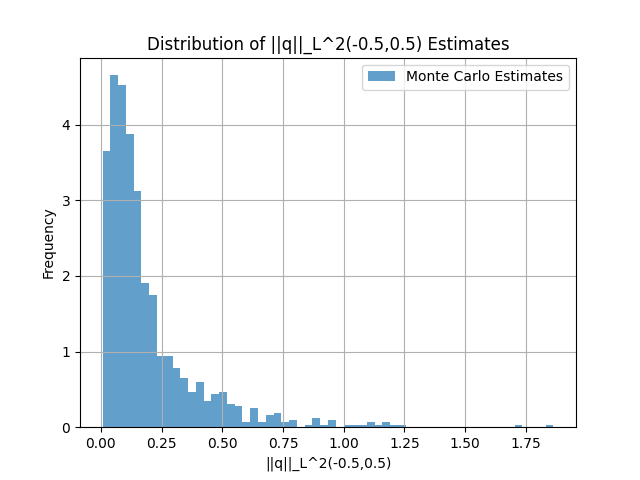
\includegraphics[height=4.5cm,width=\textwidth]{../../results/histogram_mc_estimates_seed_2026_samples_1000.png}
    \end{minipage}% <--- Nota questo percento, elimina spazi spuri
    \hfill % Spazio minimale tra le due foto
    % Seconda immagine (49% della larghezza del testo)
    \begin{minipage}[b]{0.49\textwidth}
        \centering
        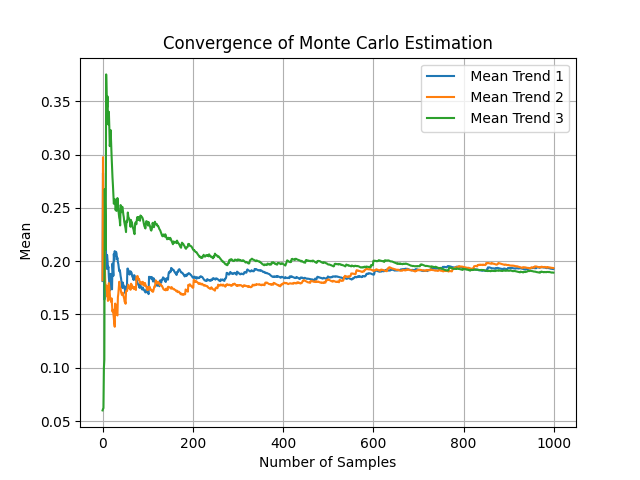
\includegraphics[height=4.5cm,width=\textwidth]{../../results/convergence_mc_seed_2026_samples_1000.png}
    \end{minipage}
    
    \vspace{-2mm} % Riduce lo spazio bianco sotto le foto
    \label{fig:conv_comparison}
\end{figure}


\section{Discussion}
One of the primary advantages of this approach is the straightforward implementation of a parallelized version. However, the main drawback remains that generating each sample for both the Monte Carlo and Multilevel Monte Carlo methods requires solving two PDEs to obtain a single realization for estimating the desired quantity. Consequently, the overall efficiency of this methodology depends on the available computer architecture.
 


\section{References}
\begin{itemize}
\item[1] Quarteroni, Sacco, Saleri, Gervasio - Matematica Numerica (4th Edition) 
\item[2] \texttt{https://en.wikipedia.org/wiki/Bessel\_function}
\item[3] \texttt{https://en.wikipedia.org/wiki/Box-Muller\_transform}
\end{itemize}

\end{document}